\chapter{Experiments}

How to structure this chapter:
\begin{enumerate}
    \item Why did we chose to go for the method: controller and see if that pose is reacheable? [DONE] 
    \item Talk about Stewart configurations, 
    \begin{itemize}
        \item which are the indices values [DONE]
        \item what these can tell us about everything [DONE]
        \item How do I want each performance index? [DONE]
        \item Show them in a graph
    \end{itemize}
    \item Given an UAV configuration (we chose triangle), analyze cable routing
    \begin{itemize}
        \item Why we choose the triangle for the UAVs configuration?
        \item How the code work, how a given cable routing has been found
        \item How can I know a configuration is mure suscettibile to be singular? Something with a jacobian?
        \item How the results before simulation and after simulation differ?
        \item Rectangle-same really unstable configuration
        \item line or diagonal results in not-feasible configurations, why? what does this mean? Geometric reasons?
    \end{itemize}
    \item Given the results of the previous step, lets analyze the first 3/5 configurations with all 6 possible uav configurations
    \begin{itemize}
        \item Expetation: triangle being the best one, if not, which one is best? Rerun step 2 and see how things change
        \item How drone attachment influences reaching the goal? Show evolution graph
    \end{itemize}
    \item Can a more spread-out hook configuration on the ground better the performance or it is irrelevant? 
    \begin{itemize}
        \item Does the answer change when the desired position is If so, it opens results to the moving hook point.further away?
        \item Show example on the top configuration and a really bad one.
        \item Is there any papers/theorem that says so?
        \item Show evolution graph
    \end{itemize}  
    \item How a configuration far away from the hook point on the ground performs?
    \begin{enumerate}
        \item Stewart: the position is reacheable with a relative small error, but it is not stable.
        \item The hook position should cover more space on the ground
        \item Is there a geometric reason/ theory for that?
    \end{enumerate} 
\end{enumerate}

\newpage

\section{Experimental methodology and evaluation framework}

%% Experimental objectives
The objective of this chapter is to evaluate how the architectural design of an ACTS influences its ability to accurately and robustly manipulate a payload. The focus is on how different cable routing strategies, UAV attachment configurations, and ground hook placements influence the overall system performance.

In fact, a configuration is considered successful if the desired payload is reached with sufficiently small position and orientation errors, all cables remain under positive tension throughout the maneuver, and the payload converges to an equilibrium without persistent oscillations.

In this chapter we will answer questions like "Which configuration gives the best payload control performance according to the theoretical indices?" and "Which configuration would I actually choose for the robot?"

%% Simulation setup.  Why simulate the controller instead of only computing the Jacobian?
The geometric and static performance indices provided in Section \ref{sec:performanceIndices} describe the instantaneous ability of a given architecture to generate payload wrenches and identify configurations that are close to kinematic singularities. However, these indices are evaluated under static or quasi-static assumptions and therefore cannot fully characterize the behavior of the closed-loop system during motion. During motion, cable directions, tensions and payload dynamics continuously evolve. Consequently, a configuration that appears favorable according to static indices may still exhibit oscillations, poor tracking or instability. Closed-loop simulation is therefore necessary to verify whether the theoretical advantages translate into practical performance.

All simulations are carried out using the MuJoCo (Multi-Joint Dynamics with Contact) physics extensions, allowing simulation of closed-loop systems, such as CDPRs and ACTSs, which is not possible in Gazebo. Another reason I switched from Gazebo to MuJoCo was the ability to model cables as tendons, which are minimum-path-length strings with wrapping and tracking, constraints \cite{mujoco_docs_237}. However, for the purpose of this thesis, the cables are treated as pure physical constraints, without stiffness or dumping.

%% Variables
The payload mass, UAV model, controller gains, drone cable lengths, simulation duration, and desired payload pose are kept constant throughout all experiments to ensure a fair comparison between diferent architectural configurations. The only variables that change from one experiment to another are the cable routing, the UAV attachment geometry, and the placement of the ground hook points.

%% Scenario A and B
Two desired payload poses are taken in considerations. In the first scenario, the desired payload orientation coincides with the world reference frame; while in the other scenario a non-zero desired orientation is imposed. This allows to analyze separately the rotational motions from the translation tracking.

%% Why did you choose Stewart as the reference?
First, the classical Stewart configuration is analyzed and used as a reference architecture due to its geometric symmetry and extensive use in the literature. In fact, if even Stewart-like performs poorly, the problem is likely the controller rather than the architecture. The remaining experiments then investigate how modifications to the ground cable routing, UAV attachment geometry, and hook placement affect both the theoretical performance indices and the closed-loop behavior of the system. This progressive analysis makes it possible to identify which geometric features have the greatest influence on payload manipulation performance.

%%The attachment points are uniformly distributed, which generally leads to good isotropy.


\section{Stewart platform baseline}
%% What should we expect from Stewart?
Thanks to its symmetrical geometry, the Stewart ground cable configuration is expected to ensure uniform torque generation in all directions while maintaining an optimal distance from singularities.
%% Which types of singularity may we encounter in general with our 6 cables on the ground?
Consequently, high values of the manipulability, capacity margin, radius of available wrench, and composite score are expected, together with a relatively high conditioning index. From a control perspective, these characteristics should result in accurate payload tracking while maintaining all cable tensions within their admissible limits.

\subsection{Numerical Verification of the Implementation}
Before comparing different ACTS architectures, one representative Stewart configuration is manually verified. The optimized cable tensions, payload wrench and UAV thrusts are recomputed directly from the governing equations presented in Chapter 2 and compared with the values returned by the implementation. This verification confirms the correctness of the numerical optimization and the controller implementation before performing the comparative study.

\subsubsection{Configuration}
Payload dimensions $2.0 \times 2.0 \times 0.2$ \\
Desired pose $p^*= [0.5, -0.5, 2.0]^\top $ \\
Desired orotation $R^* = \mathbb{I}$

\begin{table}[h]
    \centering
\begin{tabular}{lccc}
    attachment        &  points  & hook points & \\ \hline
$A_4 \equiv A_5$ &  $[0.0, 1.1, 0.0]^\top $         &   $B_4 \equiv B_9$ &  $[0.5, 0.05, 1.9]^\top $          \\
$A_6 \equiv A_7$ &  $[-0.9526, -0.55, 0.0]^\top $   &   $B_5 \equiv B_6$ &  $[-0.0237, -0.775, 1.9]^\top $    \\
$A_8 \equiv A_9$ &  $[0.9526, -0.55, 0.0]^\top $    &   $B_7 \equiv B_8$ &  $[0.9763, -0.775, 1.9]^\top $     \\ 

\end{tabular}
\end{table}
\subsubsection{Cable directions $u_i$}
Using Equation \ref{eq:cableVector}b  

\begin{table}[h]
    \centering
\begin{tabular}{cc}
 $u_4 =[-0.2245,	0.4713,	-0.8529]^\top $       & $u_7 = [-0.7100,	0.0828,	-0.6993]^\top $   \\
 $u_5 =[-0.0089,	0.7024,	-0.7117]^\top $ & $u_8 = [-0.0124,	0.1176,	-0.9930]^\top $   \\
 $u_6 =[-0.4545,	0.1047,	-0.8846]^\top $  & $u_9 = [0.2215,	   -0.2937,	-0.9299]^\top $   \\ 

\end{tabular}
\end{table}

\todo[inline]{Ground jacobian}

\todo[inline]{Cable tensions $\tau_i$}

\todo[inline]{Payload wrench $W_p$}

\todo[inline]{Required drone thrust}

\todo[inline]{Does it correspond}


\subsection{Comparison $\tau_{min}$ and $\tau_{opt}$}
%% Do the theoretical indices suggest that Stewart is a good configuration?
%% Does Stewart actually achieve the desired pose?
%% Do theory and simulation agree?

As mentioned in Section \ref{sec:highlevelarchitecture}, we evaluate two distinct tension allocation strategies:
\begin{itemize}
    \item Minimal tension strategy, in which every cable tension is imposed such that $\|\tau_i \| = \tau_{min}$.
    \item Optimal tension strategy, in which cable tensions are determined by the quadratic optimization problem in Equation \ref{eq:tension-planner-relax}
\end{itemize}

The performance indices and tracking errors under both strategies across three operational scenarios are summarized in Table \ref{tab:stewart_comparative}.

Even though being faster, the minimal tension strategy has negative consequences on the system's robustness. Pinning the tension vector to its lower limit $\tau_{\min}$ collapses the tension space from an $N$-orthotope $[\tau_{\min}, \tau_{\max}]^N$ to a single point, which linearly maps through the wrench matrix $W$ to degenerate the Available Wrench Set (AWS) into a single point \cite{yang_robust_2025}. As a result, any deviation of the desired payload wrench $W_p^*$ from this single point results in a negative capacity margin (as seen in Scenario A where $\gamma = -1.16757$). This indicates that the system is theoretically incapable of resisting external disturbances or maintaining equilibrium without violating the tension constraints.

Switching to the optimal tension allocation, allows the cable tensions to vary dynamically between $\tau_{min}$ and $\tau_{max}$. Hence, the radius of the Available Wrench increases and the capacity margin takes on a positive value ($\gamma = 5.20$). As a result, also the composite score increases.

Differently, changing the tension allocation algorithm has no effect on the conditioning index or manipulability because they are kinematic metrics that only depend on the platform's geometric position.

Although the nested structure of this optimization problem inherently increases the overall computational complexity, the primary objective of this study is offline structural and kinematic analysis rather than real-time control execution. Consequently, the computational overhead does not limit the validity of the current framework. For future real-time applications, this hierarchical formulation can be mapped to more efficient schemes.

\todo[inline]{show how position and orientation error changes overtime}
On the other hand, it is worth to notice that, since the objective function does not contain any state-tracking terms, this optimizer does not directly minimize the payload's real-time position or orientation tracking errors. 
Because of this, a spatial configuration that yields globally minimal propulsion effort does not guarantee a minimum in tracking error.

\todo[inline]{update the table based on the changes made to the code}
\begin{table}[htbp]
\centering
\small
\begin{tabular}{lcccccc}
\toprule
 & \multicolumn{2}{c}{\textbf{Scenario A} (Stable)} & \multicolumn{2}{c}{\textbf{Scenario B} (Oscillating)} & \multicolumn{2}{c}{\textbf{Scenario C} (Stable)} \\
\cmidrule(lr){2-3} \cmidrule(lr){4-5} \cmidrule(lr){6-7}
\textbf{Metric / Parameter} & $\tau_{min}$ & $\tau_{opt}$ & $\tau_{min}$ & $\tau_{opt}$ & $\tau_{min}$ & $\tau_{opt}$ \\ 
\midrule
Desired Position & \multicolumn{2}{c}{$[0.5, -0.5, 2.0]^\top$} & \multicolumn{2}{c}{$[0.5, -0.5, 2.0]^\top$} & \multicolumn{2}{c}{$[0.5, -0.5, 2.0]^\top$} \\
Desired Orientation & \multicolumn{2}{c}{$[1.0, 0.0, 0.0, 0.0]^\top$} & \multicolumn{2}{c}{$[1.0, 0.1, 0.1, 0.3]^\top$} & \multicolumn{2}{c}{$[1.0, 0.1, 0.1, 0.0]^\top$} \\
\midrule
Conditioning Index & 0.10480 & 0.09573 & 0.04361 & 0.03986 & 0.10596 & 0.09451 \\
Manipulability & 0.49089 & 0.42466 & 0.19713 & 0.17907 & 0.51002 & 0.42760 \\
Radius Avail. Wrench & 13.65493 & 20.80839 & 19.70489 & 24.23539 & 13.41358 & 17.58092 \\
Capacity Margin & -1.16757 & 5.20271 & 0.65833 & -1.70736 & -0.37528 & 4.27541 \\
Worst-case CM & 0.86285 & 0.68944 & 0.86521 & 0.86435 & 0.86385 & 0.69290 \\
Composite Score & 4.45007 & 8.90018 & 7.07614 & 7.79746 & 4.63405 & 7.51641 \\
\midrule
Position Error & 0.03150 & 0.05885 & 0.04953 & 0.05134 & 0.02904 & 0.05358 \\
Orientation Error & 0.01769 & 0.02321 & 0.22120 & 0.18969 & 0.01036 & 0.02237 \\
\bottomrule
\end{tabular}
\caption{Comparative performance indices and tracking errors for Stewart baseline configuration across Scenarios A, B, and C.}
\label{tab:stewart_comparative}
\end{table}

\todo[inline]{show performance indices of one of the scenarios over time, which one?}

Although the Stewart configuration exhibits good overall performance and provides an excellent reference architecture, the proposed ACTS differs from a classical Stewart platform because the UAV cables can be connected to the payload in several different ways. Moreover, different ground cable routings may further improve specific performance aspects such as stability, wrench generation capability, or robustness. For these reasons, the Stewart configuration is adopted as a baseline against which all alternative architectures are compared. 

An ideal ACTS architecture should remain far from singular configurations, generate payload wrenches efficiently in every direction, and maintain sufficient redundancy to accommodate disturbances while respecting cable tension limits. Consequently, all the considered performance indices should be as big as possible.

The considerations from now on will be done using the optimal tension strategy.

\todo[inline]{does the configuration chooser use tau min or tau optimal?}


\section{Ground cable routing}

\todo[inline]{Why we choose the triangle for the UAVs configuration?}

\todo[inline]{How the code work, how a given cable routing has been found}

\todo[inline]{How can I know a configuration is mure suscettibile to be singular? Something with a jacobian?}

\todo[inline]{How the results before simulation and after simulation differ?}

\todo[inline]{Rectangle-same really unstable configuration}

\todo[inline]{line or diagonal results in not-feasible configurations, why? what does this mean? Geometric reasons?}






Given a candidate pair of layouts (a payload-node layout and a ground-anchor layout, e.g. pentagon/triangle), there are usually hundreds to thousands of physically valid ways to route the 6 ground cables between the two sets of nodes. Scoring an architecture using only one (arbitrarily chosen) routing confounds two different things: how good the architecture is, and how lucky the routing choice was. This script removes that confound by exhaustively enumerating every valid routing for a given architecture, scoring each one against three necessary conditions from Sec. 2.3 of the thesis (Wrench Closure, Wrench Feasibility, Interference-Freedom), and keeping only the best surviving routing — so architectures are compared on their best achievable performance, not on chance.

It also scores every routing at every pose you supply, and keeps the
worst-case result across poses (max-min), because a routing that looks excellent at one setpoint can be nearly singular at another — Sec. 2.3's performance indices are pose-dependent, and a single-pose evaluation would be misleading.

The six ground cables are treated in isolation from the three UAV cables, justified by Sec. 2.6: the ground subsystem is modeled as its own Gough-Stewart parallel platform, with the UAVs supplying only a separate, vertical anti-gravity force.

\begin{algorithm}
\caption{Cable Routing Optimization and Architecture Ranking}
\label{alg:cable_optimization}
\begin{algorithmic}[1]

\ForAll{$(\text{payload\_layout}, \text{ground\_layout}) \text{ pairs}$}
    \State Enumerate every valid 6-cable routing via \Call{enumerate\_routings}{}
    
    \ForAll{routing}
        \ForAll{pose $\in$ test-pose set}
            \State Build $J_p$ via \Call{build\_Jp\_ground}{} \Comment{Eq. 1.7}
            \State Check Wrench Closure via \Call{score\_Jp}{} / rank test \Comment{Note 1, Sec. 2.3}
            
            \State \Comment{\textbf{Optional Checks:}}
            \State Check Wrench Feasibility via \Call{check\_wfc}{} \Comment{Eq. 1.9 / 2.35}
            \State Check Interference-Freedom via \Call{check\_ifc}{} \Comment{Eq. 2.20}
        \EndFor
        \State Record this routing's \textbf{worst-case} score across all poses
    \EndFor
    \State Keep the \textbf{best} surviving routing for this architecture
\EndFor

\State Rank all architectures by their best routing's worst-case conditioning index
\State Generate MuJoCo XML for the top 5

\end{algorithmic}
\end{algorithm}




The line and diagonal configurations approach kinematic or wrench singularities, where the cable arrangement cannot generate the desired six-dimensional wrench while maintaining positive tensions. Conversely, the Rectangle-Same configuration remains kinematically feasible but exhibits poor rotational stiffness due to its asymmetric cable pairing. As a result, although the Jacobian remains full rank, the payload develops a rocking motion that cannot be predicted by the geometric performance indices alone.

Increasing the spacing between the ground hooks enlarges the available wrench set and moves the system farther from wrench singularities, explaining the observed improvement in tracking performance.

\section{Ground hook placement}

\section{Discussion}


\newpage
\todo[inline]{Write this better}
After realizing a workable controller, which was tested using the gough stewart platform, we can proceed to consider different way to connect 6 ground cable to the platform (Figure \ref{fig:6ugvsConnections}) and the drone (Figure \ref{fig:3uavsConnections}). The same coniguration to the ground can change the stability of the system based on which point is connected to which hook on the ground.



\todo[inline]{Add the figure showing the evolution of the indices over time}
Discuss what we see and why of these results

We will compare the other configuration to this to find out if there's a better one or not. 



We can let our imaginations run wild as we create different combinations. Here, some combination whch have given interesting results or that compared to others helps us drawing conclutions.

\begin{figure}[h]
    \centering
    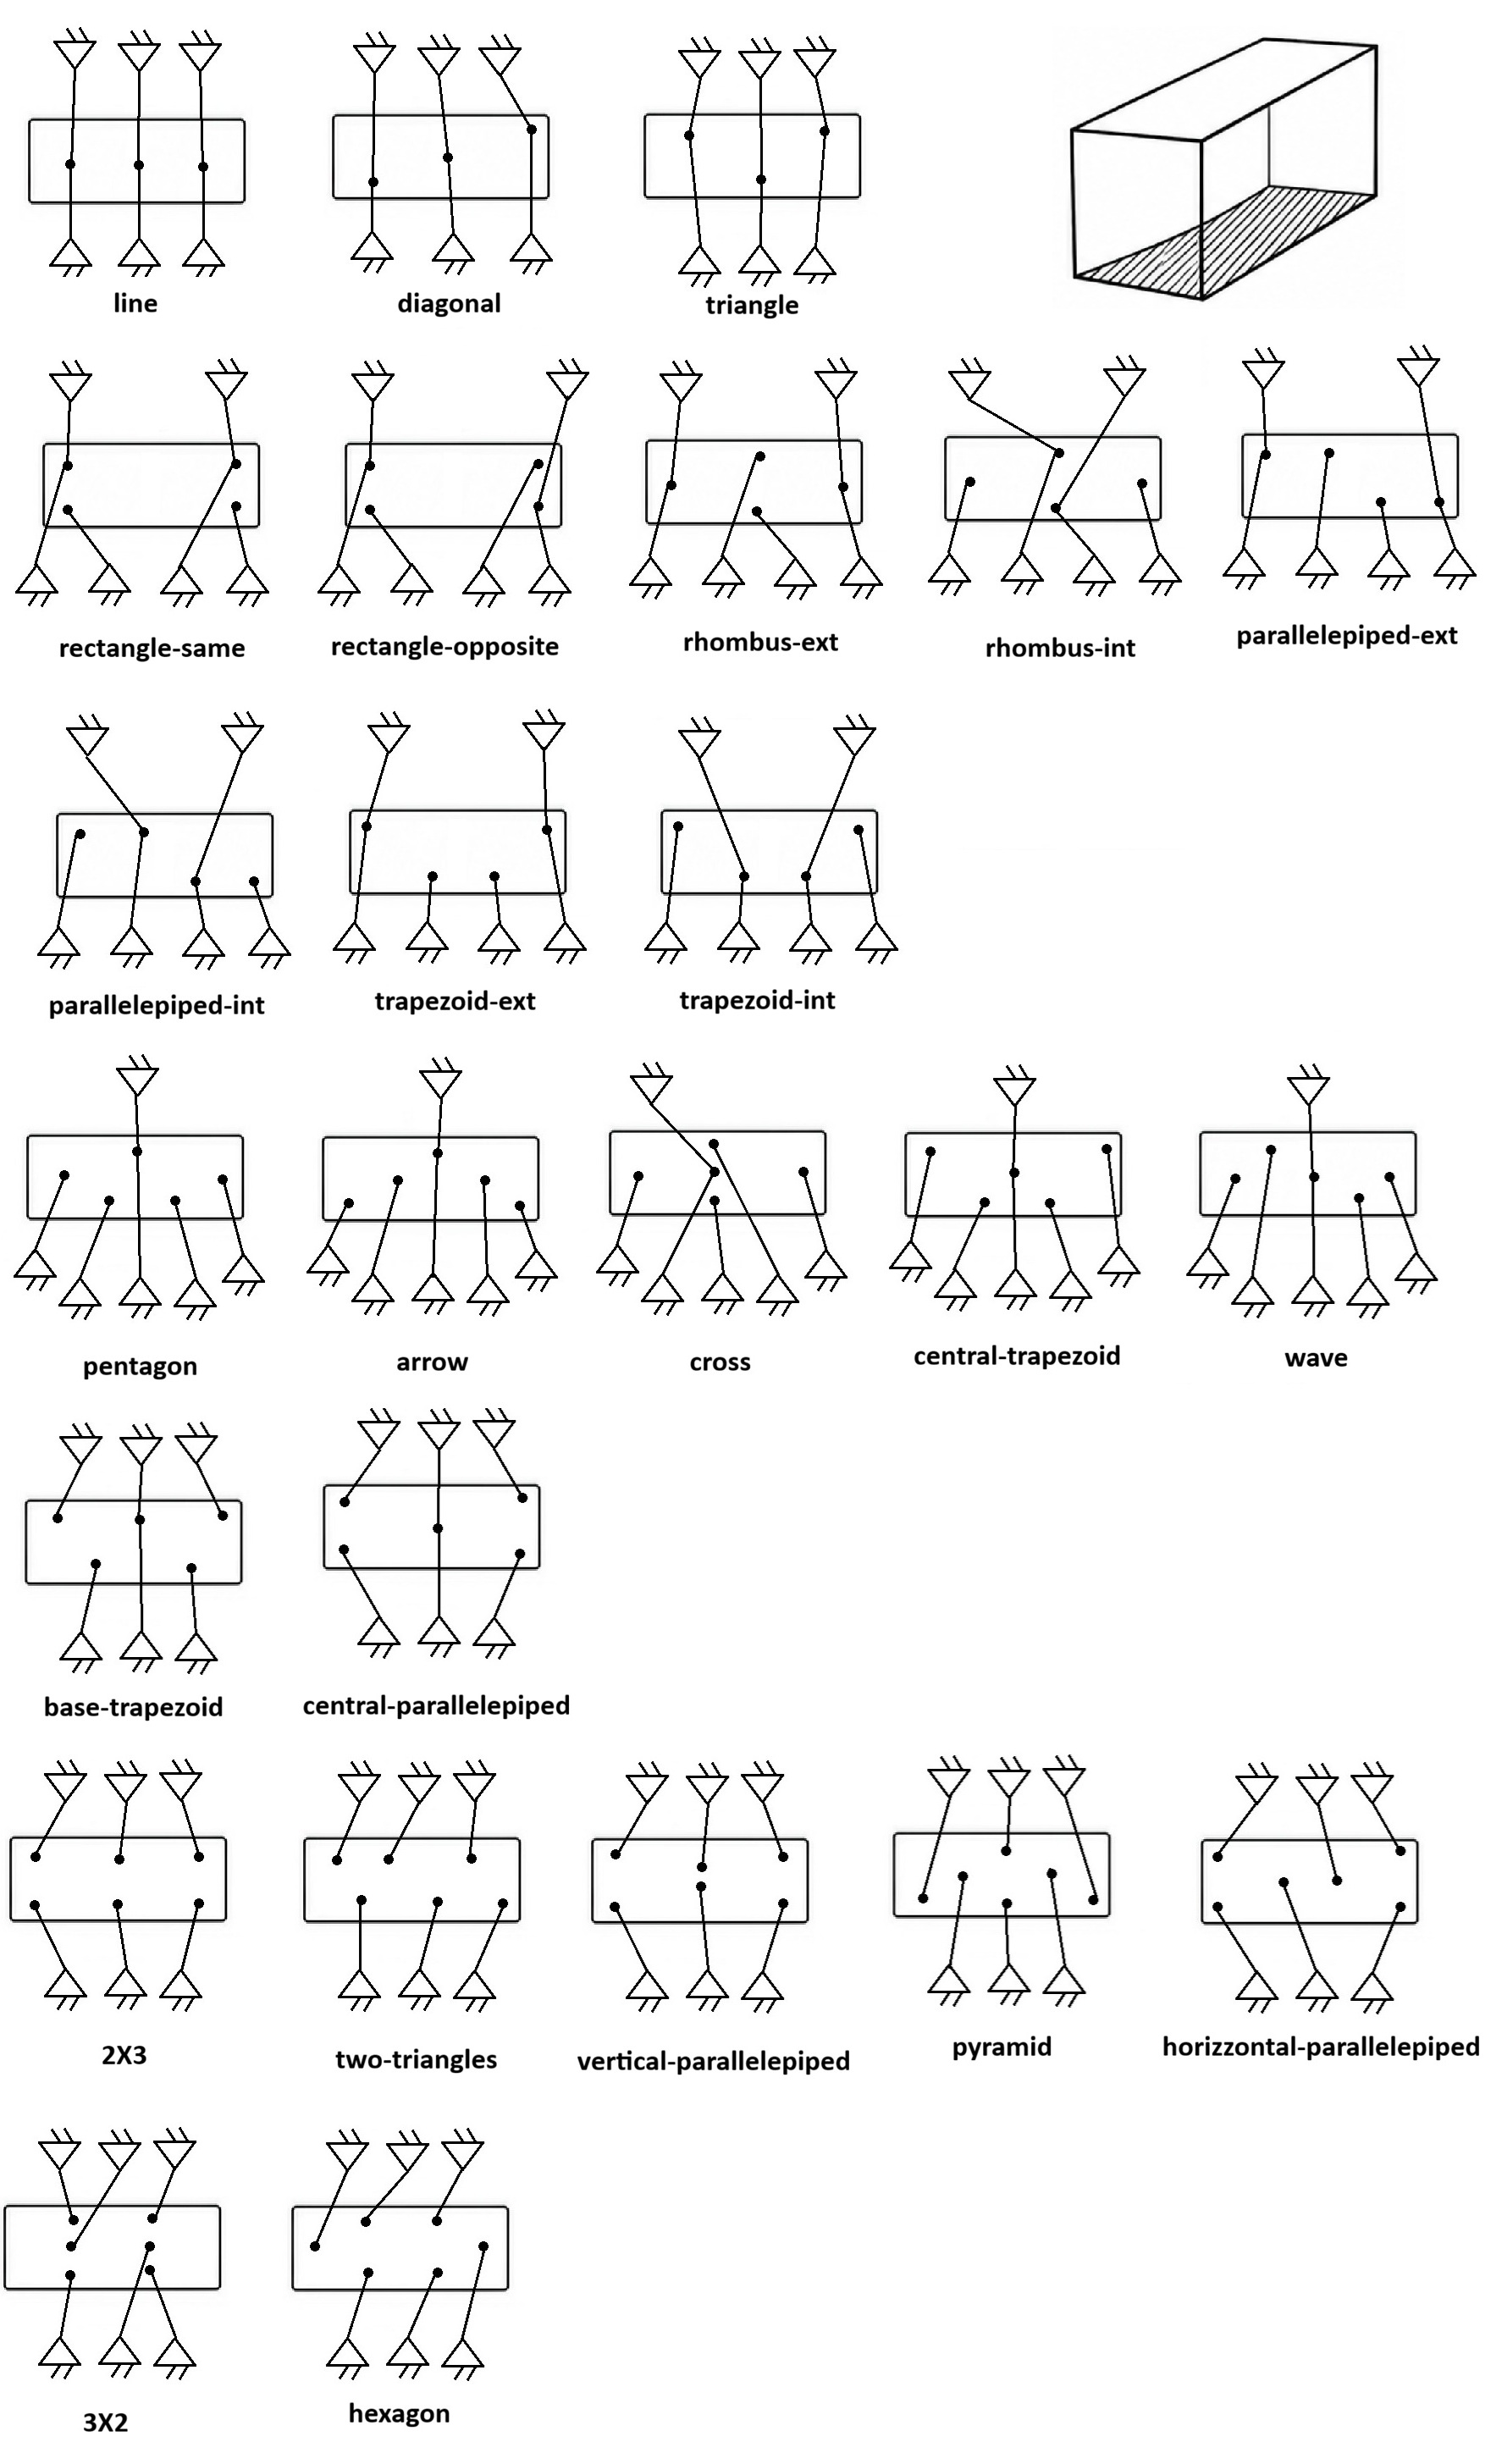
\includegraphics[width=0.6\linewidth]{images/6_ugv_config.jpeg}
    \caption{Possible 6 UGVs connections}
    \label{fig:6ugvsConnections}
\end{figure}

\begin{figure}
    \centering
    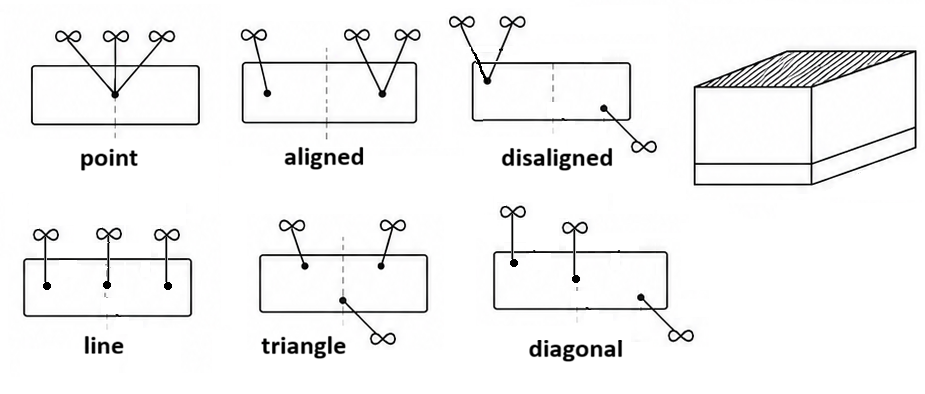
\includegraphics[width=0.6\linewidth]{images/3_uav_config.png}
    \caption{Possible 3 UAVs connection with one cable}
    \label{fig:3uavsConnections}
\end{figure}


\todo[inline]{Add link to the repository}



\todo[inline]{Rectangle-same}
The Hinge Effect: Two corners of your rectangle have double the pulling force (2 cables), while the other two corners have half the force (1 cable). This sets up a physical "rocking axis" or line of asymmetry across the platform.

Loss of Torsional Stiffness: Because the rectangle's corners are orthogonal and symmetric, pairing them up this way creates an instantaneoutexts center of rotation where the platform can twist or tilt with almost zero resistance from the cables.

Pure Kinematics vs. Statics: Your SVD code (score\_Jp) evaluates the kinematics at a perfectly static, frozen snapshot in space. It sees that the matrix is invertible and says "Feasible!". But it doesn't account for the fact that the moment a controller applies real force, this geometric asymmetry creates an unconstrained twisting motion that causes the platform to lose control.

A full-rank Jacobian is necessary but not sufficient for good closed-loop performance.

This is a very important statement.

Then explain why.

The Jacobian says

Can I generate arbitrary infinitesimal wrenches?

It does not say

Will the closed-loop system remain dynamically stable?

Your rectangle is the perfect example.

It has full rank, acceptable manipulability, acceptable conditioning

yet poor torsional stiffness, uneven load distribution, asymmetric restoring moments, oscillatory dynamics

In other words

The Jacobian is only a local kinematic property.

The simulation captures

inertia
controller
load redistribution
dynamic coupling
restoring torques

which the Jacobian completely ignores.